\documentclass[../interim.tex]{subfiles}



\begin{document}


\section{Background}

This section introduces some technical background which will likely be required as part of the project. It includes an introduction to neural networks and CNNs, a comparison of some existing object tracking and object detection algorithms and a discussion on knowledge representation and reasoning and symbolic rule learning.

\subsection{Deep Learning}

Deep neural networks (DNNs) have emerged as a very successful algorithm for machine learning; deep learning has been used to beat records in tasks such as image recognition, speech recognition and language translation\cite{deep-learning-intro}. Many different architectures have been proposed to solve various tasks, these architectures include convolutional neural networks (CNNs), which are designed to process data that come in the form of multiple arrays\cite{deep-learning-intro}, and recurrent neural networks (RNNs), which are designed to process sequences of arbitrary length\cite{def:rnn}. The following section gives a brief introduction to CNNs and describes some of their use cases.

\subsubsection{Convolutional Neural Networks}

CNNs contain three types of layers: convolution, pooling and fully connected. Units (artificial neurons) in a convolution layer are organised into feature maps. The inputs to each unit in a feature map come from the outputs of the units in a small region of the previous layer, the output of the unit is then calculated by passing the weighted sum of its inputs through an activation function such as ReLU. The set of weights, also known as a filter or kernel, is the part of the layer which is learned through backpropagation. Every unit in a feature map has the same kernel. Each feature map in a layer has its own kernel. Pooling layers reduce the size of the input by merging multiple units into one. A typical pooling operation is max-pooling, which computes the maximum of a local patch of units. Finally, in fully-connected layers (which are typically placed at the output of the CNN) every unit in a layer is connected to every unit in the previous layer. An example CNN architecture is shown in Figure~\ref{fig:example-cnn}.

\begin{figure}
  \centering
  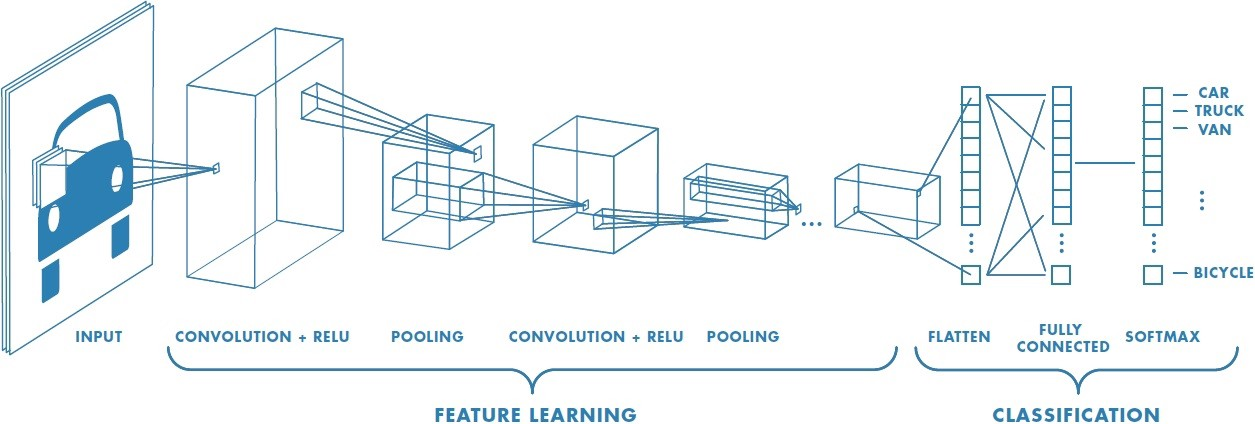
\includegraphics[width=0.8\textwidth]{cnn-example.jpg}
  \label{fig:example-cnn}
  \caption{An example of a CNN architecture. The input image is passed through a series of convolution and pooling layers before being flattened into a one-dimensional layer and passed through one final fully connected layer. The softmax classification function is then applied at the output.}
\end{figure}

CNNs have proven to be adept at a number of tasks involving images, including image classification\cite{cnn-uses:classification} and object detection\cite{cnn-uses:yolo-v3}\cite{cnn-uses:faster-r-cnn}. We explore these further in Section~\ref{section:image-proc}.


\subsection{Image Processing}
\label{section:image-proc}

\subsubsection{Object Detection}

The object detection task could formally be defined as designing a model which, when given an image, can produce a rough localisation of objects of interest in the image (in the form of a bounding box) and classify eac of these objects into a set of predefined classes. In this section we introduce two well known object detection algorithms, Faster R-CNN\cite{cnn-uses:faster-r-cnn} and You Only Look Once (YOLO)\cite{cnn-uses:yolo-v3}.

Faster R-CNN is an evolution of previous object detection algorithms, R-CNN\cite{r-cnn} and Fast R-CNN\cite{fast-r-cnn}. Faster R-CNN builds on its predecessors by adding a region proposal network (RPN) - a neural network which takes an image and produces a set of region of interest (RoI) proposals. This method of region proposal is much faster than previous algorithms (such as those used in \cite{r-cnn} and \cite{fast-r-cnn}) since it is able to make use of the GPU, as opposed to requiring the CPU. Faster R-CNN then uses a similar classifier and bounding box regressor as Fast R-CNN at the output; this section of the network also receives the feature maps from the final layer of the RPN, in this sense the initial layers of the network are shared between the region proposal section and the classifier/regressor section.

\begin{figure}
  \centering
  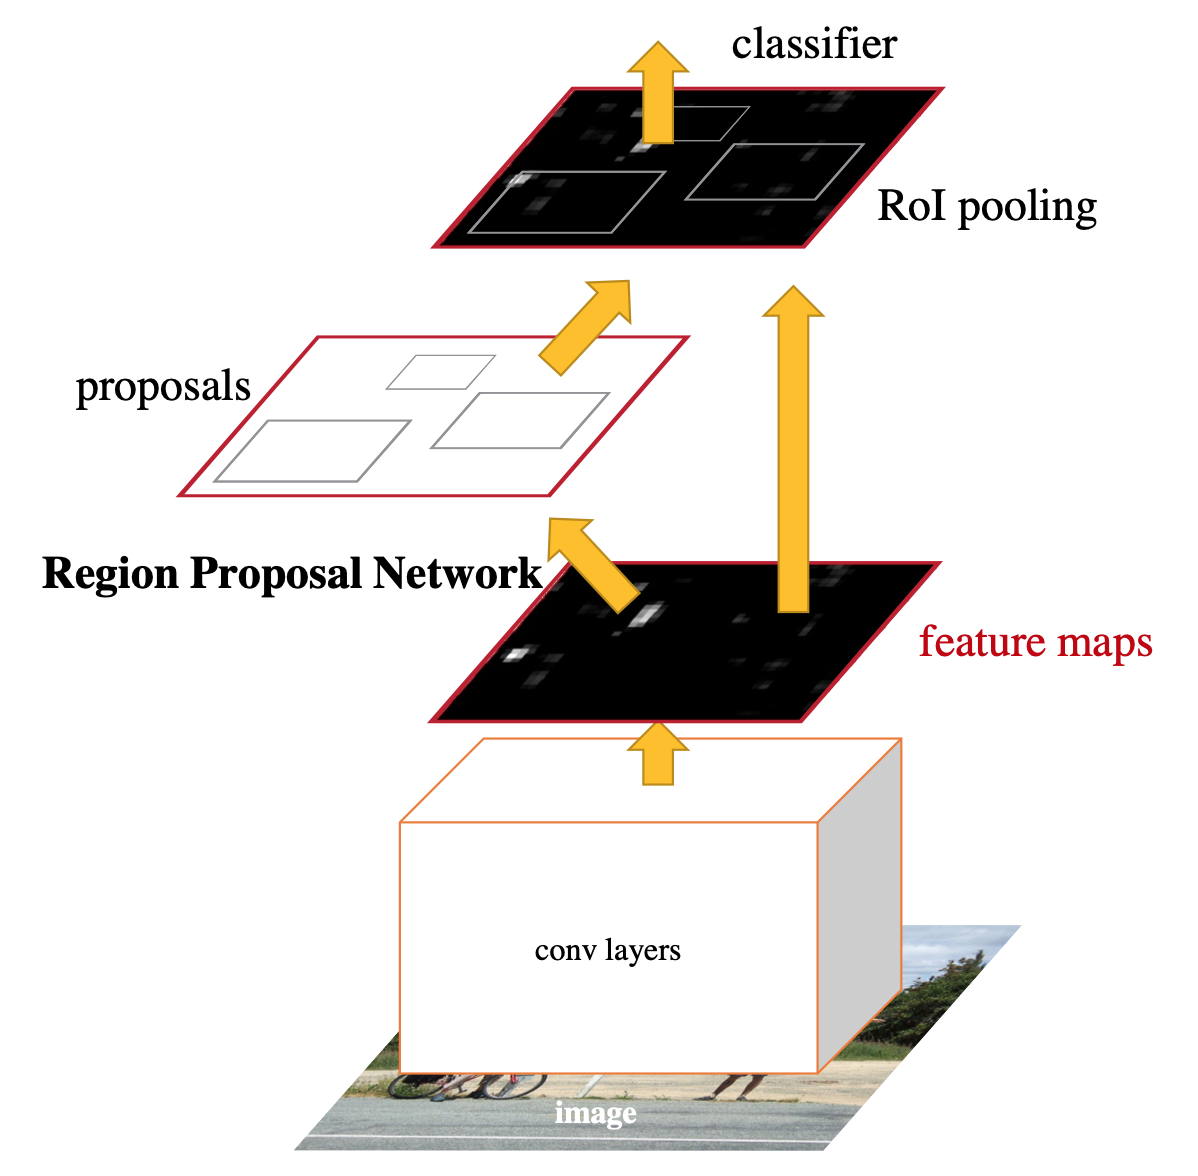
\includegraphics[width=0.4\textwidth]{faster-r-cnn.png}
  \label{fig:faster-r-cnn}
  \caption{Diagram of the Faster R-CNN architecture. One part of the network produces region proposals and another part handles bounding box regression and object classification. Figure from \cite{cnn-uses:faster-r-cnn}.}
\end{figure}

The three object detection algorithms mentioned above all work by first producing region proposals, then producing a more accurate localisation and a score for each region and finally removing any low-scoring or redundant regions. This requires the algorithm to `look' at the image multiple times (around 2000 times for R-CNN). You Only Look Once (YOLO) is a significantly more time-efficient algorithm which, as the name suggests, takes a single look at the image. A convolutional neural network is used to simultaneously predict multiple bounding boxes and the class probabilities for each box. As well as being very fast, YOLO makes fewer than half the number of background errors (where the algorithm mistakes background patches for objects) as Fast R-CNN \cite{yolo}. YOLO is, however, slightly less accurate than some of the slower methods for object detection\cite{cnn-uses:yolo-v3}.

\subsubsection{Commonly Used Metrics}


\subsubsection{Object Tracking}


\subsection{Knowledge Representation and Reasoning}

\subsubsection{The Event Calculus}

\subsubsection{Answer Set Programming}

\subsubsection{Symbolic Rule Learning}

\subsubsection{Ontologies}


\end{document}
